%%%%%%%%%%%%%%
%  COSTANTI  %
%%%%%%%%%%%%%%
%COMANDI DA UTILIZZARE PER TUTTI I DOCUMENTI
% In questa prima parte vanno definite le 'costanti' utilizzate da due o più documenti.

%COMANDI TABELLE
\newcommand{\rowcolorhead}{\rowcolor[HTML]{00ACC1}} %intestazione 
\newcommand{\rowcolorlight}{\rowcolor[HTML]{E0f7fa}} %righe chiare/dispari
\newcommand{\rowcolordark}{\rowcolor[HTML]{80DEEA}} %righe scure/pari
\newcommand{\colorhead}{\color[HTML]{FFFFFF}} %testo intestazione
\newcommand{\colorbody}{\color[HTML]{000000}} %testo righe


%%%%%%%%%%%%%%
%  FUNZIONI  %
%%%%%%%%%%%%%%

% Serve a dare la giusta formattazione al codice inline
\newcommand{\code}[1]{\flextt{\texttt{#1}}}

% Genera automaticamente la pagina di copertina
\newcommand{\makeFrontPage}{
  % Declare new geometry for the title page only.
  \newgeometry{top=4cm}
  
  \begin{titlepage}
  \begin{center}

\begin{center}
  \centerline{
\includegraphics[scale=0.24]{StyleLatex/logo_home.png}}
\end{center}
  
  \vspace{1cm}

  \begin{Huge}
  \textbf{\DocTitolo{}} \\
  \end{Huge}

  \vspace{9pt}  
  
  \begin{tabular}{l|l}
  	\textbf{Nome Gruppo} & WalkAndBuy \\
  	\textbf{Componenti} & Canovese Marco 1094135\\
  	& Zanellato Federico 1094134\\

  \end{tabular}

  \vspace{30pt}
  

  \end{center}
  \end{titlepage}
  
  % Ends the declared geometry for the titlepage
  \restoregeometry
}
%\documentclass[a4paper, oneside, openany]{book}
\documentclass[10pt,a4paper]{extarticle}

%**************************************************************
% Importazione package
%************************************************************** 
\usepackage{graphbox}
% permette di modificare i margini
%\usepackage[top=3.1cm, bottom=3.1cm, left=2.2cm, right=2.2cm]{geometry}
%\usepackage[a4paper]{../../common/style/geometry} %TODO
\usepackage[a4paper, top=2cm, bottom=2.8cm]{geometry}
\usepackage{booktabs} %lista item nelle tabelle
% specifica con quale codifica bisogna leggere i file
\usepackage[utf8]{inputenc}

%indice con i puntini
\usepackage{tocloft}
\renewcommand\cftsecleader{\cftdotfill{\cftdotsep}}



% necessario per risolvere il problema del carattere invisibile per l'a capo
\DeclareUnicodeCharacter{00A0}{ } %?

% per scrivere in italiano e in inglese;
% l'ultima lingua (l'italiano) risulta predefinita
\usepackage[english, italian]{babel}

% imposta lo stile italiano per i paragrafi
\usepackage{parskip}

% fornice elenchi numerati in ordine inverso
\usepackage{etaremune}

\usepackage{caption}

% comandi per l'appendice
\usepackage{appendix}
%\renewcommand\appendixtocname{Appendici} %We really need it?

% import euro symbol
\usepackage{eurosym}

% numera anche i sottoparagrafi
\setcounter{secnumdepth}{5}

% elenca anche i sottoparagrafi nell'indice
\setcounter{tocdepth}{5}

% permetti di definire dei colori
\usepackage[usenames,dvipsnames]{color}

% permette di usare il comando "paragraph" come subsubsubsection!
\usepackage{titlesec}

% permette di inserire le immagini/tabelle esattamente dove viene usato il
% comando \begin{figure}[H] ... \end{figure}
% evitando che venga spostato in automatico
\usepackage{float}

% permette l'inserimento di url e di altri tipi di collegamento
\usepackage[colorlinks=true]{hyperref}

\hypersetup{
    colorlinks=true, % false: boxed links; true: colored links
    citecolor=black,
    filecolor=black,
    linkcolor=black, % color of internal links
    urlcolor=Maroon  % color of external links
}

% permette al comando \url{...} di andare a capo a metà di un link
\usepackage{breakurl}

% immagini
\usepackage{graphicx}

% permette di riferirsi all'ultima pagina con \pageref{LastPage}
\usepackage{lastpage}

% tabelle su più pagine
\usepackage{longtable}

% per avere dei comandi in più da poter usare sulle tabelle
\usepackage{booktabs}

% tabelle con il campo X per riempire lo spazio rimanente sulla riga
%\usepackage{tabularx}

% TABELLE 
% tabelle su più pagine
\usepackage{longtable}

% per avere dei comandi in più da poter usare sulle tabelle
\usepackage{booktabs}

% multirow per tabelle
\usepackage{multirow}

% definisci un nuovo tipo di colonna C che permette di andare a capo con \newline
% e centrata
\usepackage{array}
\usepackage{ragged2e}
%\newcolumntype{P}[1]{>{\RaggedRight\hspace{0pt}}p{#1}}
\newcolumntype{C}[1]{>{\centering\let\newline\\\arraybackslash\hspace{0pt}}m{#1}}

% colore di sfondo per le celle
\usepackage[usenames,dvipsnames,svgnames,table]{xcolor}

% tabelle con il campo X per riempire lo spazio rimanente sulla riga
\usepackage{tabularx}


% personalizza l'intestazione e piè di pagina
\usepackage{fancyhdr}

% permette di inserire caratteri speciali
\usepackage{textcomp}

% permette di aggiustare i margini e centrare tabelle e figure
\usepackage{changepage}

%Permette di includere i grafici a barre
%IMPORTANTE: deve essere caricato prima di /pgfgantt altrimenti causa conflitto
%\usepackage{pgfplots}

% permette di includere i diagrammi Gantt
% su Ubuntu non si può installare il pacchetto, deve essere in modello/
%\usepackage{../../modello/pgfgantt}

% permette di includere i grafici a torta
%\usepackage{../../modello/pgf-pie}

% necessario per pgf-pie
\usepackage{tikz}

% permette i path delle immagini con gli spazi
\usepackage{grffile}

% ruota le immagini
\usepackage{rotating}

% permetti di calcolare le larghezze facendo calcoli
\usepackage{calc}


\fancypagestyle{plain}{
	% cancella tutti i campi di intestazione e piè di pagina
	\fancyhf{}

	\lfoot{
		\DocTitolo{} \ - \textit{\DocRedazione{} \ -  \DocAnno{}}
	}
	\rfoot{Pagina \thepage{} di \pageref{LastPage}}

	% Visualizza una linea orizzontale in cima e in fondo alla pagina
	\renewcommand{\headrulewidth}{0pt}	
	\renewcommand{\footrulewidth}{0.3pt}
}
\pagestyle{plain}

% allarga l'header a tutta la pagina
%\fancyhfoffset[L]{\oddsidemargin + \hoffset + 1in}
%\fancyhfoffset[R]{\evensidemargin + \marginparwidth - \marginparsep}

% Per inserire del codice sorgente formattato

\usepackage{listings}

\lstset{
  extendedchars=true,          % lets you use non-ASCII characters
  inputencoding=utf8,   % converte i caratteri utf8 in latin1, richiede 
  %\usepackage{listingsutf8} anzichè listings
  basicstyle=\ttfamily,        % the size of the fonts that are used for the 
  %code
  breakatwhitespace=false,     % sets if automatic breaks should only happen at 
  %whitespace
  breaklines=true,             % sets automatic line breaking
  captionpos=t,                % sets the caption-position to top
  commentstyle=\color{mygreen},   % comment style
  frame=none,               % adds a frame around the code
  keepspaces=true,            % keeps spaces in text, useful for keeping 
  %indentation of code (possibly needs columns=flexible)
  keywordstyle=\bfseries,     % keyword style
  numbers=none,               % where to put the line-numbers; possible values 
  %are (none, left, right)
  numbersep=5pt,              % how far the line-numbers are from the code
  numberstyle=\color{mygray}, % the style that is used for the line-numbers
  rulecolor=\color{black},    % if not set, the frame-color may be changed on 
  %line-breaks within not-black text (e.g. comments (green here))
  showspaces=false,           % show spaces everywhere adding particular 
  %underscores; it overrides 'showstringspaces'
  showstringspaces=false,     % underline spaces within strings only
  showtabs=false,             % show tabs within strings adding particular 
  %underscores
  stepnumber=5,               % the step between two line-numbers. If it's 1, 
  %each line will be numbered
  stringstyle=\color{red},    % string literal style
  tabsize=4,                  % sets default tabsize
  firstnumber=1      % visualizza i numeri dalla prima linea
}

% Permetti di utilizzare il grassetto per i caratteri Typewriter (per es. il 
%font di \code{...} e \file{...})
\usepackage[T1]{fontenc}
\usepackage{lmodern}


%package added
\usepackage{amsmath}

\usepackage{amsfonts}

%%%%%%%%%%%%%%
%  COSTANTI  %
%%%%%%%%%%%%%%

% In questa prima parte vanno definite le 'costanti' utilizzate soltanto da questo documento.
% Devono iniziare con una lettera maiuscola per distinguersi dalle funzioni.

\newcommand{\DocTitolo}{Relazione progetto TecWeb}

\newcommand{\DocRedazione}{WineNot}

\newcommand{\DocAnno}{Anno 2017/2018}

\title{\textbf{Relazione progetto TecWeb}}
\author{WalkAndBuy}

\date{11 Settembre 2018}

\begin{document}

%\maketitle

\makeFrontPage

\tableofcontents

\newpage

\section{Introduzione}

Lo scopo del progetto è quello di creare un e-commerce gestito dall’Associazione Agricoltori del Camposampierese, la quale a fronte dell'inarrestabile concorrenza dei grandi colossi del commercio online ha deciso di favorire un servizio dedicato agli agricoltori e commercianti del territorio.\\
Il sito web permette infatti alle aziende del territorio, previo accordo con l’Associazione, di promuovere e vendere i propri prodotti online. \\
Il servizio offerto è limitati ai cittadini residenti nei comuni ove l’Associazione ha dei soci attivi. 
I prodotti vendibili devono essere afferenti ad una delle macro categorie previste, ovvero:
\begin{itemize}
	\item frutta e Verdura;
	\item carne e Pesce;
	\item formaggi;
	\item conserve e Uova;
	\item vino e Bevande.
\end{itemize}
Ogni articolo viene presentato mediante:
\begin{itemize}
	\item titolo;
	\item sintetica descrizione;
	\item un’immagine rappresentativa;
	\item la quantità venduta;
	\item il prezzo di rivendita al netto di eventuali sconti promozionali applicati.
\end{itemize}
I commercianti abilitati possono modificare gli articoli da essi pubblicati.\\

Gli utenti una volta autenticati possono consultare il catalogo online, aggiungere e rimuovere articoli dal carrello e una volta selezionati tutti gli articoli di loro interesse, concludere l’ordine. \\
Hanno inoltre a disposizione una pagina in cui possono visualizzare i singoli ordini effettuati.\\

L’Associazione viene registrata tramite un account amministrativo ed ha potere di modificare qualsiasi articolo e di assegnare o revocare il ruolo di “azienda” ad un singolo utente. 
\newpage
\section{Descrizione dei tipi di utente}
In questa sezione verranno analizzate le diverse tipologie di utenti che possono usufruire del sito, cosi da avere un chiaro target su cui costruire le varie pagine del sito.
\subsection{Utente non autenticato}
	Si tratta dell'utente che non è iscritto al sito, può essere di passaggio o comunque supponiamo questo tipo di utente non abbia alcuna relazione con il nostro sito, il nostro obiettivo quindi è fare in modo che l'utente resti positivamente colpito dal sito e venga invogliato ad iscriversi.\\
	Per ottenerlo abbiamo deciso di minimizzare il livello di profondità del sito, rendendo sempre chiaro all'utente dove si trova tramite titoli chiari e ben visibili e un menù di categoria sempre presente.\\
	Gli utenti non autenticati hanno la possibilità di visionare tutti i prodotti, tuttavia viene richiesta la registrazione se si vuole procedere con l'acquisto.

\subsection{Utente autenticato - Standard}
	Con utente autenticato si intende un utente che ha deciso di effettuare la registrazione presso il nostro sito, esistono due tipologie di utenti autenticati, Standard e Azienda, questa differenza è designabile solamente dall'amministratore. \\
	L'utente standard è un utente normale, senza particolari privilegi o esigenze, il suo obiettivo è accedere al sito e acquistare i prodotti presenti in vetrina. Per raggiungere il suo scopo, oltre alla possibilità di visionare i diversi prodotti gli è possibile aggiungerli al carrello, visionare quest'ultimo con possibilità di modifica delle quantità.\\
	E' presente inoltre una pagina di riepilogo degli acquisti, in cui l'utente può visualizzare lo storico degli acquisti effettuati!\\\\
	Ovviamente, essendosi registrato, l'utente ha accesso alla propria pagina profilo, in cui può aggiornare o aggiungere dati relativi alla propria persona.

\subsection{Utente autenticato - Azienda}
Un utente segnato come \textbf{Azienda} può, oltre che avere tutte le funzionalità dell'utente standard, inserire nuovi articoli e modificare i propri.\\ 	
L'interfaccia quindi sarà uguale a quella degli altri due utenti, a differenza dell'header in cui ci sarà un link che permetterà all'utente di arrivare al form di inserimento di un nuovo articolo.\\
Oltre a questo, nella pagina di dettaglio di un articolo, nel caso in cui questo sia stato inserito dall'azienda loggata, quest'ultima, tramite l'apposito bottone, ha la possibilità di accedere al form di modifica di quel determinato articolo.
	
\subsection{Utente autenticato - Amministratore}
L'amministratore è un utente speciale, rappresenta il consorzio, di conseguenza ha pieni poteri.\\
In particolare, tramite un link inserito nella pagina del profilo, ha la possibilità di accedere al pannello amministrativo in cui ha la possibilità di modificare la tipologia di un utente registrato, da \textit{Azienda} a \textit{Standard} o viceversa

\newpage

\section{Analisi delle pagine}
In questa sezione verranno analizzate tutte le pagine del sito con le diverse azioni che possono essere effettuate e i privilegi in base alla tipologia di utente che vi accede.\\
Verranno esposte in base alle tipologie di account che vi accedono, dall'utente non autenticato fino all'amministratore.
\subsection{Pagine di accesso e registrazione}
Queste due pagine sono accessibili solo da utenti non autenticati, permettono all'utente di effettuare l'accesso se si è già registrati, oppure iscriversi se non lo si è già.
\subsubsection{Accedi}
Semplice schermata di Login, formato da un form centrato, viene richiesta l'\textbf{e-mail} e la \textbf{Password}.\\
tramite link è possibile passare direttamente alla pagina di registrazione.
	\begin{figure}[H]
	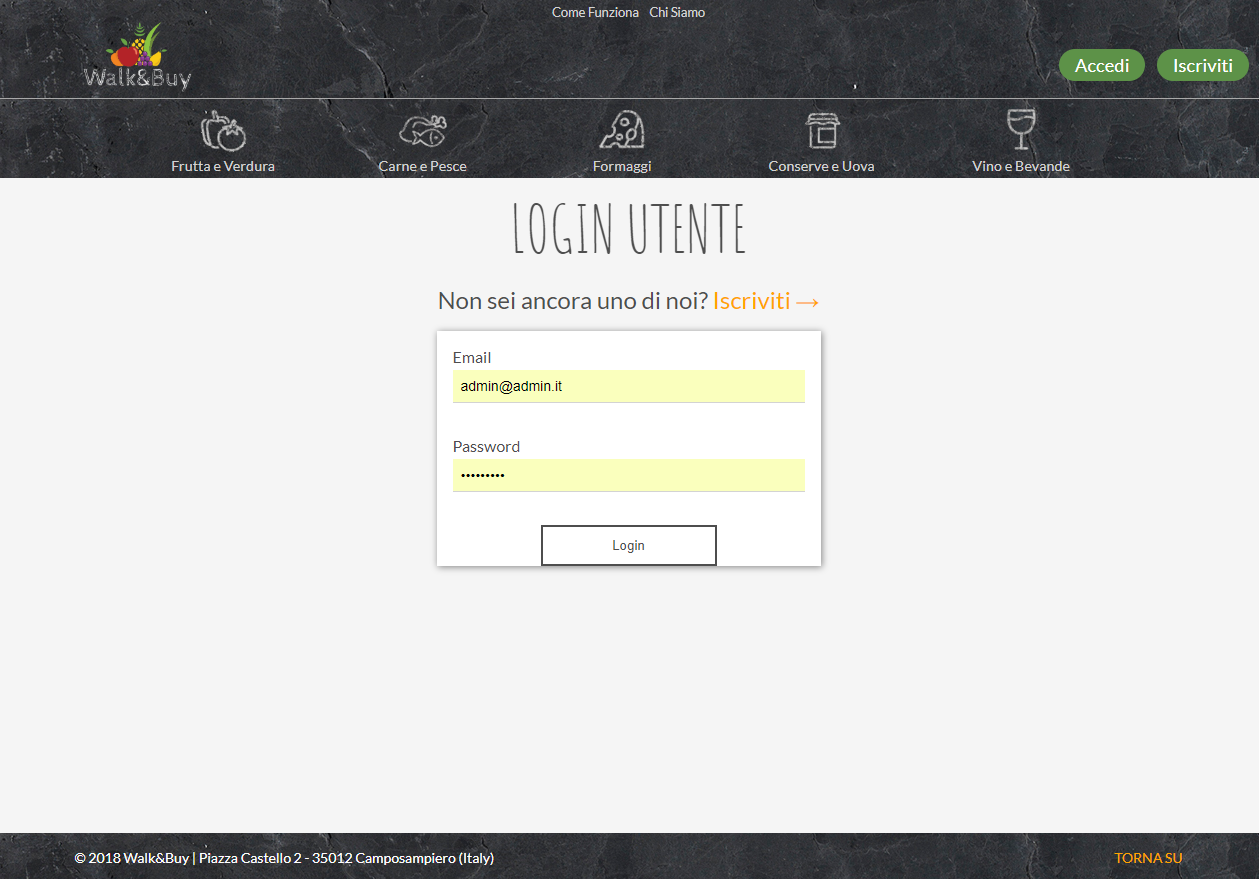
\includegraphics[width=\linewidth]{res/img/login}
	\caption{Pagina di Login}
	\label{Pagina di Login}
\end{figure}
\newpage
\subsubsection{Iscriviti}
La pagina di iscrizione contiene un form un po' più corposo, in cui l'utente deve inserire i propri dati al fine di creare un profilo che gli permetterà di navigare e acquistare liberamente dal sito.
\begin{figure}[H]
	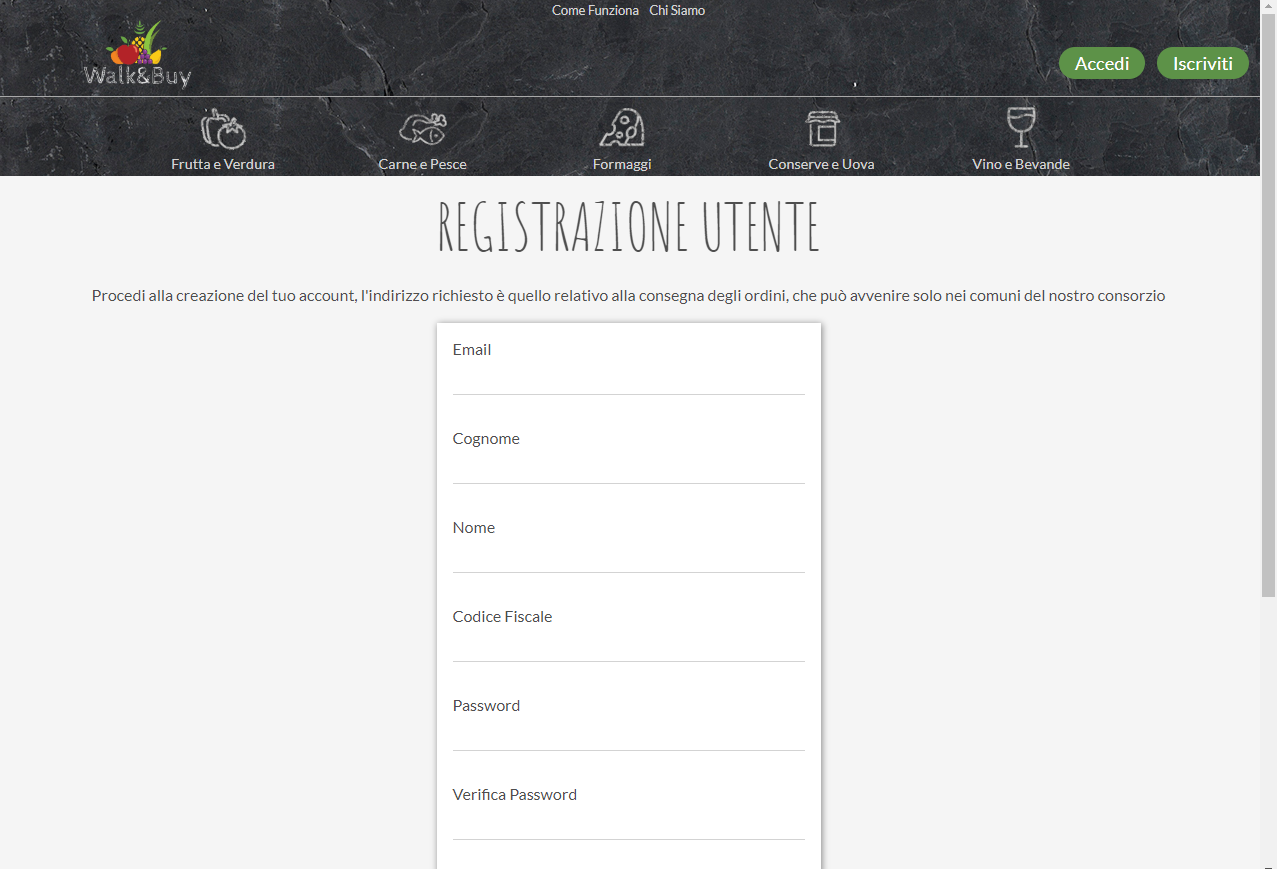
\includegraphics[width=\linewidth]{res/img/registrazione}
	\caption{Pagina di registrazione}
	\label{Pagina di registrazione}
\end{figure}
\subsection{Pagine accessibili da tutti}
	\subsubsection{Header}
		Menzione particolare va fatta all'header, presente in ogni singola pagina per rendere la navigazione chiara e semplice, essendo comune a tutte le pagine verrà esposta all'inizio.
		nella parte più alta dell'header sono presenti due link che riportano alle omonime pagine informative:
		\begin{itemize}
			\item \textit{Chi siamo};
			\item \textit{Come funziona}.
		\end{itemize}
	
		Nella parte centrale troviamo :
		\begin{itemize}
			\item logo del sito, posto in alto a sinistra, che, nel caso di click, riporta alla \textit{Homepage};
			\item (da utente non autenticato) link per accedere alle pagine di \textit{Login} e \textit{Registrazione}, posti in alto a destra;
			\item (da utente autenticato, di qualsiasi tipo) pagina di carrello, profilo, ordini. Queste si possono trovare in alto a destra, identificabili tramite apposite icone.
		\end{itemize} 
		
		Nella parte bassa invece, abbiamo un menù fisso orizzontale, che riporta le macro-categorie visitabili.
		\begin{itemize}
			\item \textit{Frutta e Verdura};
			\item \textit{Carne e Pesce};
			\item \textit{Formaggi};
			\item \textit{Conserve e Uova};
			\item \textit{Vino e Bevande}.
		\end{itemize}
	\begin{figure}[H]
		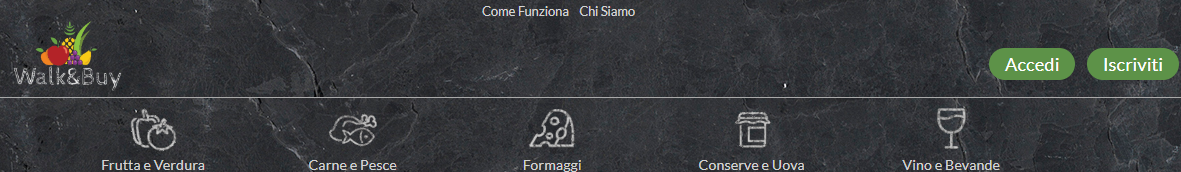
\includegraphics[width=\linewidth]{res/img/HeaderNA}
		\caption{Header visto da utente non autenticato}
		\label{Header visto da utente non autenticato}
	\end{figure}
	\begin{figure}[H]
		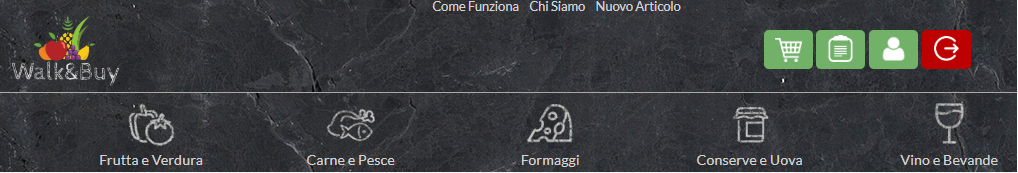
\includegraphics[width=\linewidth]{res/img/HeaderAut}
		\caption{Header visto da utente autenticato}
		\label{Header visto da utente autenticato, azienda in questo caso}
	\end{figure}
	\subsubsection{Footer}
	Il footer, come l'header, è presente in tutte le pagine.\\
	Riporta solamente dati anagrafici del consorzio proprietario del sito e sulla destra un comodo link \textbf{Torna su} per ritornare in testa alla pagina in modo immediato.
	
	\subsubsection{Homepage}
	Landing page del sito, è raggiungibile da qualsiasi punto del sito cliccando sul logo in alto a sinistra.\\
	Presenta in breve il servizio offerto e rende disponibili alcune immagini promozionali.

	\subsubsection{Macro-Categoria}
	Questa pagina contiene una lista di tutte le categorie facenti parte della macro-categoria scelta (ad es: macro-categoria \textit{Frutta e Verdura}, la pagina relativa contiene una lista di prodotti della categoria \textit{Frutta} e un'altra con i prodotti della categoria \textit{Verdura}  (\textit{Fig. 3})).\\
	Di questi prodotti è possibile vedere il \textbf{titolo di categoria}; una lista limitata di prodotti di esempio con tanto di \textbf{foto}, \textbf{nome prodotto}, \textbf{prezzo} (e relativo \textbf{sconto} se presente), e \textbf{quantità}.\\

	\begin{figure}[H]
		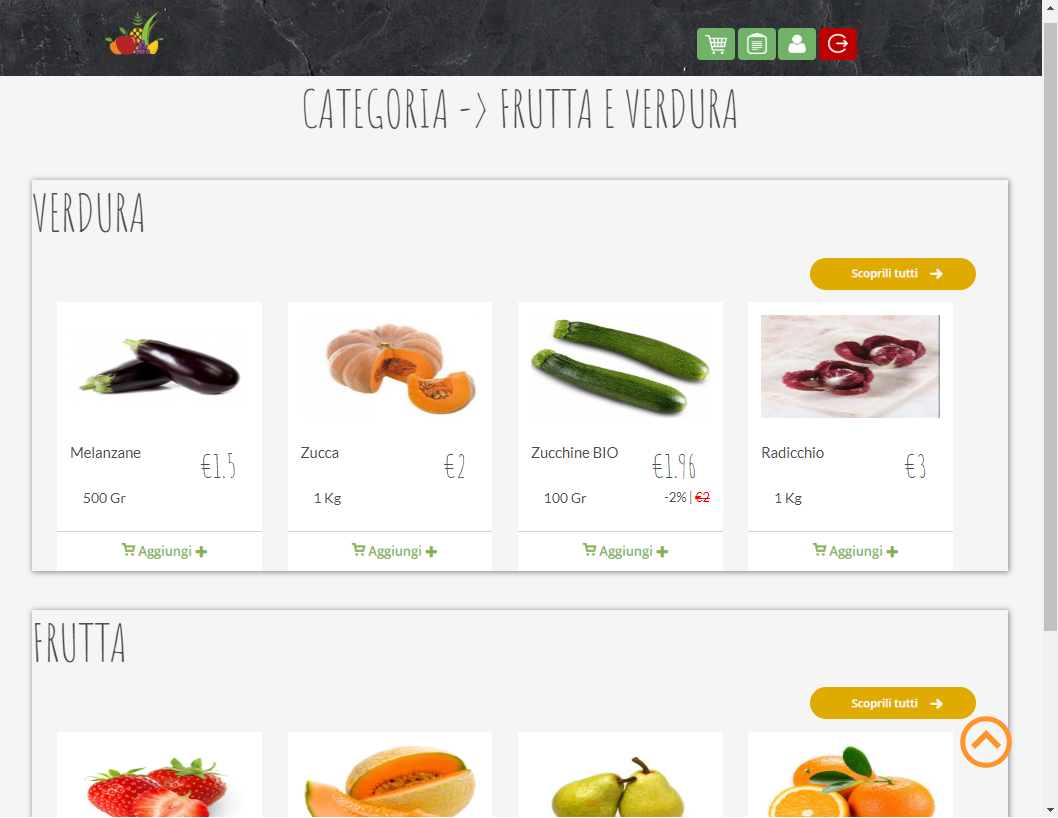
\includegraphics[width=\linewidth]{res/img/Macro-cat}
		\caption{Esempio pagina macro-categoria, in questo caso \textit{Frutta e Verdura}}
		\label{Pagina Macro-categoria}
	\end{figure}
	Come si può vedere dalla figura tramite il bottone "\textit{Scoprili tutti}" è possibile ampliare la categoria scelta e visualizzare tutti i prodotti disponibili, entrando nella pagina di \textit{Sotto-categoria}.\\
	E' possibile inoltre, se si è autenticati, aggiungere direttamente il prodotto al carrello oppure entrare nella pagina di \textit{Singolo prodotto}.
	
	\subsubsection{Sotto-categoria}
	Si accede a questa pagina tramite bottone "\textit{Scoprili tutti}" in una delle  presente nella pagina \textit{Macro-categoria}.\\
	Molto simile alla pagina precedente, tuttavia in questa schermata è possibile vedere tutti i prodotti disponibili di una determinata sotto-categoria.\\
	Anche qui è possibile (se autenticati) aggiungere un prodotto al carrello oppure aprire la pagina di \textit{Singolo prodotto} per visionare ulteriori dati sul prodotto.
	\begin{figure}[H]
		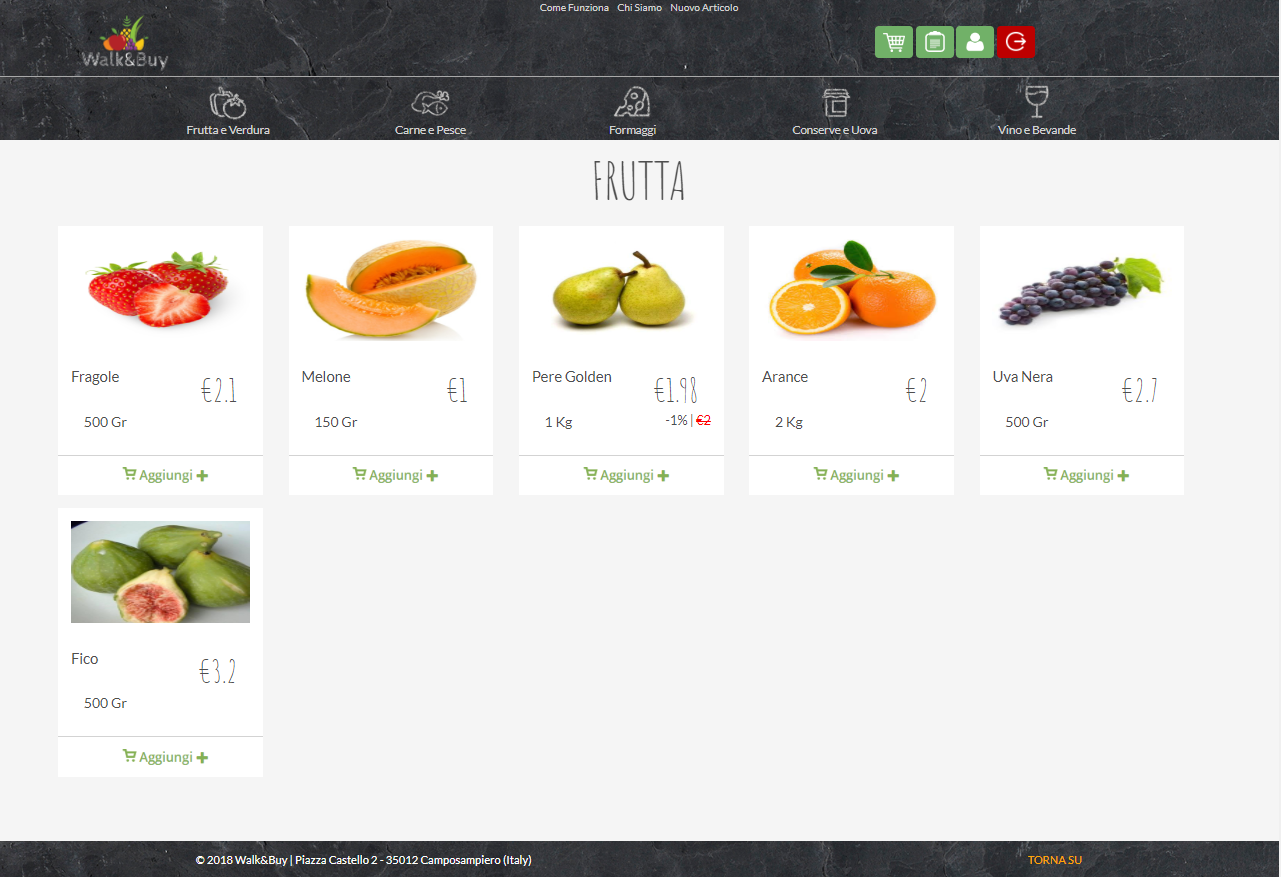
\includegraphics[width=\linewidth]{res/img/sotto-cat}
		\caption{Esempio pagina sotto-categoria, in questo caso \textit{Frutta}}
		\label{Pagina Sotto-categoria}
	\end{figure}

	\subsubsection{Chi siamo e Come funziona}
	Queste due pagine contengono informazioni utili riguardanti rispettivamente :il consorzio e lo scopo del sito (\textit{Chi siamo}) e come funziona quest'ultimo, con disponibilità del servizio e orari di assistenza clienti (\textit{Come funziona}).
	 
\subsection{Pagine accessibili da utenti autenticati}
	\subsubsection{Carrello}
	Raggiungibile cliccando sull'icona del carrello posta in alto a destra previa autenticazione.\\
	La pagina si presenta con un riquadro centrale che presenta i prodotti presenti nel carrello.\\
	Si ha la possibilità di entrare nella pagina relativa al singolo prodotto, in cui sono presenti maggiori dettagli, oppure è possibile aggiungere o rimuovere unità di prodotto, cliccando \textbf{+} o \textbf{-}; quando si è soddisfatti dei prodotti inseriti nel carrello, tramite il pulsante \textit{Procedi con l'acquisto} è possibile procedere ed inserire l'ordine, l'indirizzo di consegna quello utilizzato in fase di registrazione.
	\begin{figure}[H]
		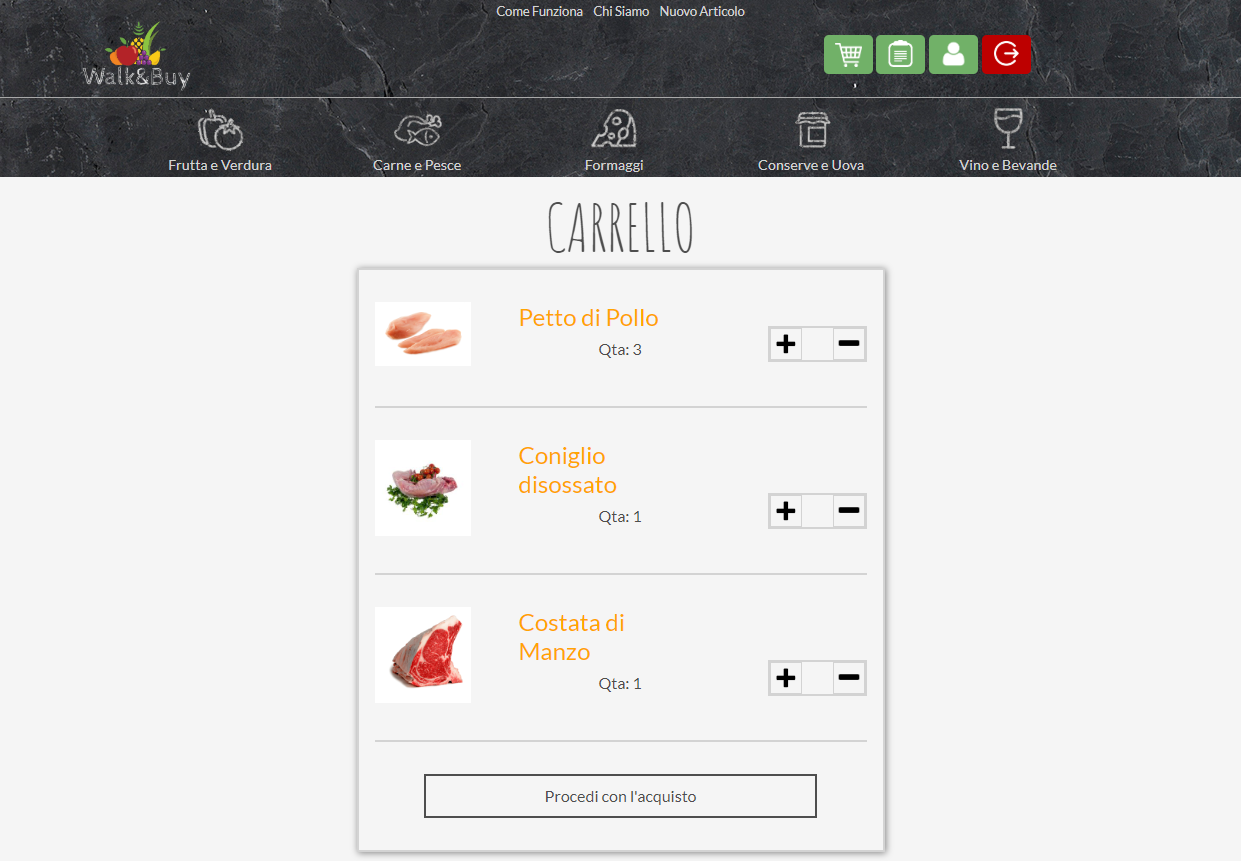
\includegraphics[width=\linewidth]{res/img/carrello}
		\caption{Pagina del carrello}
		\label{Carrello}
	\end{figure}
	\subsubsection{Profilo}
	Vi è possibile accedervi dall'icona di un omino stilizzato posta in alto a destra previa autenticazione.\\
	La pagina del profilo si presenta con un box centrale contenente i dati anagrafici dell'utente, in basso a destra del box è presente un link "\textit{Modifica profilo}", il quale permette di accedere alla pagina di modifica dei valori.\\
	\textbf{NOTA:} se si è amministratori, in questa pagina, sopra il box, è possibile cliccare sul link ed accedere all'area amministrativa.
	
	\subsubsection{Ordini}
	Vi è possibile accedervi dall'icona di un blocco note posta in alto a destra previa autenticazione.\\
	La pagina degli ordini si presenta con una lista di box contenenti le specifiche dei diversi ordini, con la data, il totale speso, lo stato, il metodo di pagamento e di spedizione.\\
	In basso a destra di ogni box è presente un link "\textit{Dettagli ordine}" che rimanda alla pagina di dettaglio, in cui sono presenti i prodotti acquistati riferiti all'ordine scelto.
	
	\subsubsection{Singolo prodotto}
	Si raggiunge cliccando l'immagine del prodotto nelle pagine di \textit{Categoria} e \textit{sotto-categoria}, oppure dal nome dell'articolo nel \textit{carrello} o nel \textit{dettaglio ordine}.\\ Permette di visualizzare più nel dettaglio un singolo prodotto, con la possibilità di aggiungerlo al carrello.\\
	La pagina si presenta con l'immagine del prodotto sulla sinistra e una colonna di informazioni sulla destra.\\
	\textbf{NOTA:} se si è proprietari del prodotto (o amministratori) è possibile, tramite il link posto sotto all'immagine, accedere al form di modifica dell'articolo.
	\begin{figure}[H]
		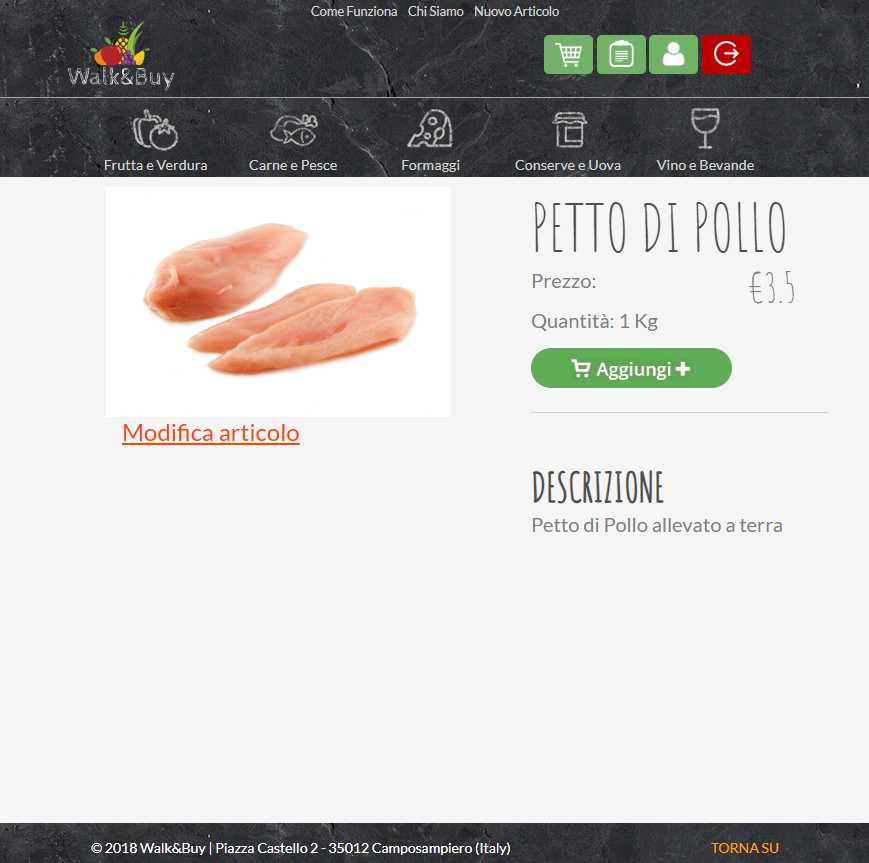
\includegraphics[width=\linewidth]{res/img/sing-prod+}
		\caption{Pagina singolo articolo (Petto di pollo)}
		\label{Pagina singolo articolo}
	\end{figure}
	
	\subsubsection{Inserisci Articolo}
	Raggiungibile \textit{SOLO} se si è un utente di tipo azienda (o amministratore), tramite un link posto sopra l'header.\\ Questa pagina permette di compilare un form e inserire un articolo nel database del sito e renderlo disponibile agli utenti per l'acquisto.\\
	L'amministratore ha la possibilità di modificare o rimuovere gli articoli se non pertinenti o se presentano dati poco pertinenti.


\section{Design}
	Abbiamo adottato uno stile moderno e semplice. Abbiamo preso spunto da vari siti e-commerce di ortaggi, sfruttando principalmente colori quali il verde, l'arancione, color lavagna per header e footer e il grigio per mantenere un tocco di eleganza.\\ Abbiamo cercato di mantenere un buon livello di contrasto per permettere la navigazione anche ad utenti con particolari problemi di vista.

\subsection{Accessibilità}
Il design si è basato su accessibilità e responsività, per la prima sono state adottate le seguenti scelte:
\begin{itemize}
	\item Il layout è responsive, cosi da essere accessibile da qualsiasi tipo di dispositivo e impedendo scroll orizzontali.
	\item Il menù è presente in tutte le pagine, in caso di scroll della pagina (e JS attivato) resta fisso nella parte alta, lasciando però solo logo e pulsanti di interesse, cosi da non essere troppo opprimente.
	\item I link sono chiaramente visibili e il loro scopo è chiaro e non permette ambiguità.
	\item La profondità del sito è stata limitata, cosi da permettere all'utente di avere ben chiara la struttura già dal primo utilizzo, questo permette una navigazione più immediata e una sensazione di maggior sicurezza.
	\item Si sono scelti due tipologie di font, uno per titoli e prezzi, accattivante, per attirare l'attenzione su questi due punti, il secondo, più chiaro e con meno grazie, per la descrizione ed altri campi, cosi facendo si affatica meno la lettura e si rende il tutto più fruibile.
	\item Nel footer è stato posto un link "Torna su" per tornare facilmente all'header completo. In caso di JS attivo, questo link segue l'utente in ogni punto dello scroll. 
\end{itemize}
\subsection{Responsive}

Il sito è stato sviluppato tenendo in considerazione le diverse dimensioni di dispositivo utilizzabile, risulta infatti perfettamente fruibile anche con schermi più piccoli, testato fino a 400px senza avere effetti disastrosi.

\subsection{Verifica}
Le verifiche e i test sono stati effettuati sui principali browser, quali \textit{Internet Explorer v10-11}, \textit{Microsoft Edge v16-v17},  \textit{Google Chrome v68},
\textit{Mozilla Firefox} e \textit{Safari}, non è stato riscontrato nessun problema di navigazione e/o visualizzazione.
\section{Progettazione tecnica}
La progettazione tecnica suddivide il sito in parte front-end e back-end.
\subsection{Front-end}

La parte front-end si occupa nello specifico nella visualizzazione delle varie parti del sito.\\
Le tecnologie utilizzate sono HTML, CSS e Javascript.\\
Il codice è stato scritto interamente dal team.

\subsubsection{HTML}

Lo standard utilizzato per HTML è HTML5 in quanto quest’ultimo è supportato da tutti i recenti browser sia utilizzati su client desktop che mobile. 
Nel corso dello sviluppo però si è constatato che l’impiego effettivo delle funzioni aggiuntive di HTML5 rispetto a versioni precedenti è stato limitato alla validazione dei form.

\subsubsection{CSS}
Lo standard utilizzato per il CSS è CSS3, sempre cercando di utilizzare attributi supportati dalla maggioranza dei browser.\\
Gli aspetti più rilevanti del CSS sono:
\begin{itemize}
	\item Utilizzo di misure relative, in particolare \textbf{rem} per rendere il contenuto della pagina variabile, ed essendo relativo al documento html permette di tenere conto anche delle preferenze utente legate al browser.
	\item I file .CSS sono stati diversificati in base alla pagina e prendono il nome di \textit{pagina} .CSS, e vengono importati solamente all'apertura di quest'ultima, cosi da evitare complessità e pesantezza in un unico file.\\Class e ID comuni sono stati salvati nel file \textit{Common.CSS}.
\end{itemize}

\subsubsection{JavaScript}
Il linguaggio JavaScript è stato utilizzato solamente per migliorare l'esperienza utente in caso di ridimensionamento della pagina o scroll vari.\\ Il sito risulta totalmente navigabile anche senza JavaScript attivo.
\newpage
\subsection{BackEnd}
Il back-end si occupa della parte server del sito, viene suddiviso in due parti: DB in MySQL e PhP.

\subsubsection{Database MySQL}
Il DB è stato progettato dal team dopo aver effettuato un'attenta analisi dei requisiti, il risultato è il seguente:
\begin{figure}[H]
	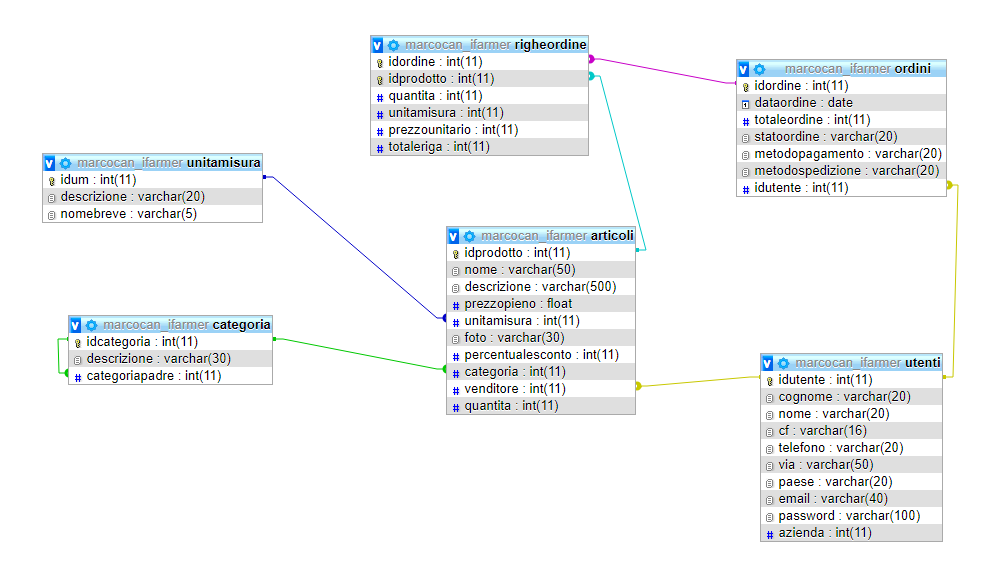
\includegraphics[width=\linewidth]{res/img/DB}
	\caption{Database}
	\label{Database Walk And Buy}
\end{figure}
Il database è stato opportunamente normalizzato e i campi sono correttamente identificati.

\subsubsection{PhP}
Il progetto è sviluppato secondo il pattern MVC (Model-View-Controller) le cui fondamenta sono state apprese principalmente mediante la consultazione di materiale reperibile sul web ed in particolare grazie al tutorial “The PHP Practitioner” il quale ha fortemente inspirato lo sviluppo del progetto.
\begin{itemize}
	\item Nella \textbf{root} del progetto è presente il file \textit{routes.php} che associa il controller a seconda della pagina richiesta dal server.
	\item In \textbf{App} troviamo le seguenti directory:
	\begin{itemize}
		\item \textbf{Controller}: al cui interno sono reperibili tutti i controller sviluppati secondo il pattern MVC e si occupano dell’elaborazione dei dati prelevati dal database e li rendono disponibili alle varie view mediante HTML e CSS.
		\item \textbf{Models}: due classi definite nel progetto, in particolare Articoli per la descrizione dei singoli articoli in vendita e Users per la definizione degli utenti.
		\item \textbf{Views}: file che contengono principalmente codice HTML che permette la visualizzazione delle informazioni elaborate dai controller.
	\end{itemize} 
	\item In\textbf{Core} troviamo le classi fondamentali che permettono il funzionamento dell'applicativo secondo il pattern MVC:
	\begin{itemize}
		\item \textbf{App}: per la condivisione e inizializzazione di variabili condivise.
		\item \textbf{Bootstrap}: esegue il caricamento delle classi descritte sopra e crea le variabili condivise mediante l’utilizzo di App.
		\item \textbf{Request}: si occupa di gestire il recupero dei dati inviati al server con chiamate \textit{GET} o \textit{POST}.
		\item \textbf{Router}: permette di effettuare il match tra ciò che viene richiesto al server e le routes disponibili, effettuando quindi il collegamento tra pagina richiesta e controller.
		\item \textbf{Session}: si occupa della gestione della sessione.
	\end{itemize} 
\end{itemize}

\subsubsection{Accessibilità}
è stato tenuto conto dell'accessibilità per soddisfare la navigazione da parte di tutte le tipologie di utenti. Vengono elencate di seguito le principali attività che hanno permesso il raggiungimento di un livello soddisfacente di accessibilità:
\begin{itemize}
	\item Tutte le immagini sono provviste di attributo \textit{alt} e \textit{title} con descrizione significativa.
	\item è stato utilizzato l'attributo \textit{tabindex} per permettere la navigazione da tastiera.
	\item Si è evitato l'uso di tabelle, preferendo \textit{div}  dal contenuto lineare e semplice.
	\item sono stati utilizzati \textit{label} ed aiuti testuali per aiutare l'utente a compilare i form.
	\item è implementata la \textit{Pagina 404} in caso di rotta non riconosciuta, per non disorientare l'utente.
\end{itemize}
Per testare l'accessibilità sono stati effettuati test con \textit{Total Validator}, in particolare è stato utilizzato per testare la correttezza e l'accessibilità dei form secondo lo standard WCAG2-A.



\section{Suddivisone del lavoro}
Di seguito viene riportata la suddivisione del lavoro:
\begin{itemize}
	\item Marco Canovese:
	\begin{itemize}
		\item gestione struttura delle directory;
		\item PhP;
		\item parte di HTML;
		\item parte del DB MySql;
		\item parte dei form;
		\item testing accessibilità del sito.
	\end{itemize}
\end{itemize}

\begin{itemize}
	\item Federico Zanellato:
	\begin{itemize}
		\item parte HTML;
		\item CSS;
		\item parte del DB MySql;
		\item parte dei form;
		\item relazione;
		\item JavaScript.
	\end{itemize}
\end{itemize}

\end{document}